\begin{frame}[label=digital_twin]
    \frametitle{Validation: Simulating a Real System}
    \begin{columns}
        \begin{column}{0.65\textwidth}
            \centering \vspace*{5pt}
            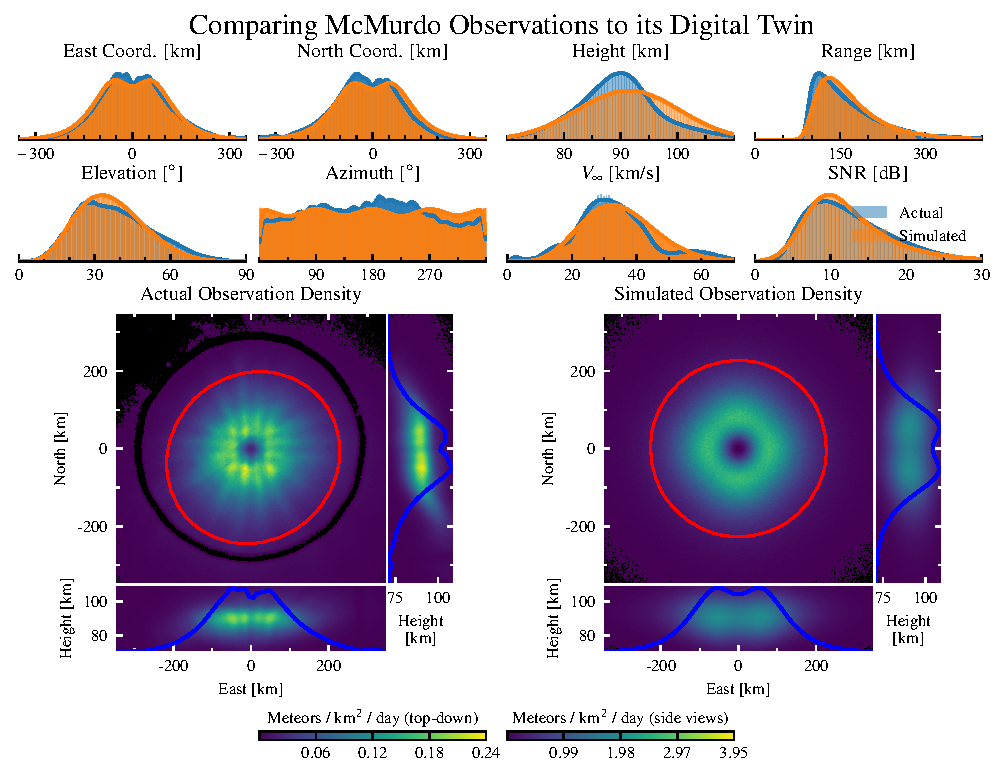
\includegraphics[height=\textheight - 1.25cm]{img/comparitive_hists.pdf}
        \end{column}
        \begin{column}{0.4\textwidth}
            \small
            \textbf{But:} does this tool match reality? \\ ~ \\ 
            
            Let's find out by simulating a real system: 

            ~ \\ 
            The \alert{McMurdo monostatic meteor radar}
            \begin{itemize}
                \item 4+ years of observations available (N=1.8e7)
                \item Reliable, well-understood
            \end{itemize} 

            Sampling 100 billion meteors gives similar observation distributions!
            \begin{itemize}
                \item[\(\blacktriangleright\)] Accurate digital twin
                \item[\(\blacktriangleright\)] N=1.1e7 (2.46 years equivalent) 
            \end{itemize}
        \end{column}
    \end{columns}
\end{frame}